\documentclass{article}
\usepackage[utf8]{inputenc}
\usepackage[T1]{fontenc}
\usepackage{tikz}
\usepackage{amssymb}

% Definição do símbolo branco
\newcommand{\blank}{\square}

\usetikzlibrary{automata, positioning, arrows, shapes}

\begin{document}

\begin{center}
\textbf{MT Decisora para $L = \{ w \in \{a,b\}^* \mid n_a(w) = n_b(w) \}$}
\vspace{1cm}
% Não retirar comentários, nem mesmo este
% Nossa sintaxe de transições: símbolo / símbolo movimento (ex: a / X D).
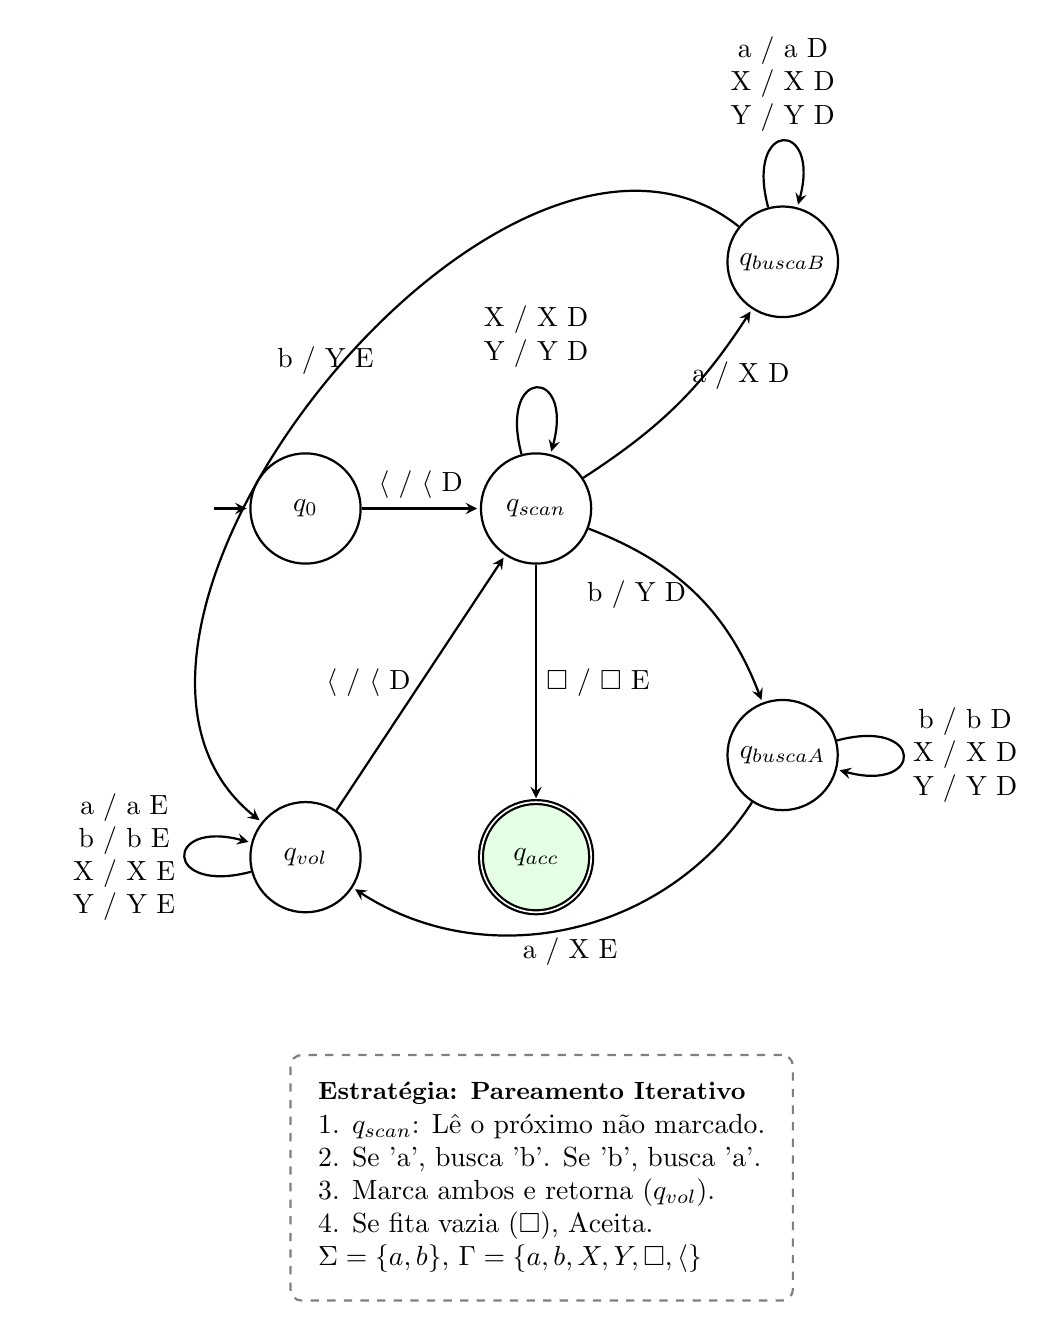
\begin{tikzpicture}[
    ->,
    >=stealth,
    shorten >=1pt,
    auto,
    node distance=3cm,
    thick,
    state/.style={circle, draw, minimum size=1.4cm, thick, fill=white},
    accept/.style={double, circle, draw, minimum size=1.4cm, thick, fill=green!10},
    initial text= % não precisa de nome
  ]

  % --- POSICIONAMENTO DOS ESTADOS ---
  
  % Estado inicial que lida com a marcação de início
  \node[state, initial] (q0) {$q_{0}$};
  
  % Estado central que decide o que buscar
  \node[state, right=1.5cm of q0] (qscan) {$q_{scan}$};
  
  % Estado que volta a cabeça para o início
  \node[state, below=of q0] (qvol) {$q_{vol}$};
  
  % Estado de aceitação
  \node[accept, below=of qscan] (qacc) {$q_{acc}$};
  
  % Buscadores
  \node[state, above right=of qscan] (qbuscaB) {$q_{buscaB}$};
  \node[state, below right=of qscan] (qbuscaA) {$q_{buscaA}$};

  % --- TRANSIÇÕES ---

  % 1. Inicialização: Pula o marcador de início '<'
  \path (q0) edge node {$\langle$ / $\langle$ D} (qscan);

  % 2. Scanner (Decisor)
  % Se ler X ou Y, ignora (já pareado).
  % Se ler 'a', marca X e vai buscar 'b'.
  % Se ler 'b', marca Y e vai buscar 'a'.
  % Se ler Branco, aceita (tudo pareado ou vazio).
  \path (qscan)
  % loop com label deslocado para cima
  edge[loop above] node[align=center, above=4pt] {X / X D \\ Y / Y D} (qscan)
  
  % seta para qbuscaB, com leve curvatura e label deslocado
  edge[bend right=12] node[above right=2pt] {a / X D} (qbuscaB)

  % seta para qbuscaA
  edge[bend left=24] node[left] {b / Y D} (qbuscaA)

  % seta para qacc
  edge node[right] {$\blank$ / $\blank$ E} (qacc);

  % 3. Busca por B (foi lido um 'a', precisa de um 'b')
  % Pula 'a' (outros as), 'X' e 'Y'.
  % Se achar 'b', marca 'Y' e volta.
  % (Se achar branco, trava/rejeita implicitamente)
  \path (qbuscaB) edge[loop above] node[align=center] {a / a D \\ X / X D \\ Y / Y D} (qbuscaB)
                  edge[bend right=90] node[above] {b / Y E} (qvol);

  % 4. Busca por A (foi lido um 'b', precisa de um 'a')
  % Pula 'b' (outros bs), 'X' e 'Y'.
  % Se achar 'a', marca 'X' e volta.
  \path (qbuscaA) edge[loop right] node[align=center] {b / b D \\ X / X D \\ Y / Y D} (qbuscaA)
                  edge[bend left=45] node[below] {a / X E} (qvol);

  % 5. Retorno (Rewind)
  % Volta tudo até bater no marcador de início '<'
  \path (qvol) edge[loop left] node[align=center] {a / a E \\ b / b E \\ X / X E \\ Y / Y E} (qvol)
               edge node[left] {$\langle$ / $\langle$ D} (qscan);

  % --- LEGENDA ---
  \node[draw=black!50, dashed, rounded corners, inner sep=10pt, align=left] 
  at (3, -8.5) {
    \small
    \textbf{Estratégia: Pareamento Iterativo}\\
    1. $q_{scan}$: Lê o próximo não marcado.\\
    2. Se 'a', busca 'b'. Se 'b', busca 'a'.\\
    3. Marca ambos e retorna ($q_{vol}$).\\
    4. Se fita vazia ($\blank$), Aceita.\\
    $\Sigma = \{a, b\}$, $\Gamma = \{a, b, X, Y, \blank, \langle\}$
  };

\end{tikzpicture}
\end{center}

\end{document}